\documentclass[1p]{elsarticle_modified}
%\bibliographystyle{elsarticle-num}

%\usepackage[colorlinks]{hyperref}
%\usepackage{abbrmath_seonhwa} %\Abb, \Ascr, \Acal ,\Abf, \Afrak
\usepackage{amsfonts}
\usepackage{amssymb}
\usepackage{amsmath}
\usepackage{amsthm}
\usepackage{scalefnt}
\usepackage{amsbsy}
\usepackage{kotex}
\usepackage{caption}
\usepackage{subfig}
\usepackage{color}
\usepackage{graphicx}
\usepackage{xcolor} %% white, black, red, green, blue, cyan, magenta, yellow
\usepackage{float}
\usepackage{setspace}
\usepackage{hyperref}

\usepackage{tikz}
\usetikzlibrary{arrows}

\usepackage{multirow}
\usepackage{array} % fixed length table
\usepackage{hhline}

%%%%%%%%%%%%%%%%%%%%%
\makeatletter
\renewcommand*\env@matrix[1][\arraystretch]{%
	\edef\arraystretch{#1}%
	\hskip -\arraycolsep
	\let\@ifnextchar\new@ifnextchar
	\array{*\c@MaxMatrixCols c}}
\makeatother %https://tex.stackexchange.com/questions/14071/how-can-i-increase-the-line-spacing-in-a-matrix
%%%%%%%%%%%%%%%

\usepackage[normalem]{ulem}

\newcommand{\msout}[1]{\ifmmode\text{\sout{\ensuremath{#1}}}\else\sout{#1}\fi}
%SOURCE: \msout is \stkout macro in https://tex.stackexchange.com/questions/20609/strikeout-in-math-mode

\newcommand{\cancel}[1]{
	\ifmmode
	{\color{red}\msout{#1}}
	\else
	{\color{red}\sout{#1}}
	\fi
}

\newcommand{\add}[1]{
	{\color{blue}\uwave{#1}}
}

\newcommand{\replace}[2]{
	\ifmmode
	{\color{red}\msout{#1}}{\color{blue}\uwave{#2}}
	\else
	{\color{red}\sout{#1}}{\color{blue}\uwave{#2}}
	\fi
}

\newcommand{\Sol}{\mathcal{S}} %segment
\newcommand{\D}{D} %diagram
\newcommand{\A}{\mathcal{A}} %arc


%%%%%%%%%%%%%%%%%%%%%%%%%%%%%5 test

\def\sl{\operatorname{\textup{SL}}(2,\Cbb)}
\def\psl{\operatorname{\textup{PSL}}(2,\Cbb)}
\def\quan{\mkern 1mu \triangleright \mkern 1mu}

\theoremstyle{definition}
\newtheorem{thm}{Theorem}[section]
\newtheorem{prop}[thm]{Proposition}
\newtheorem{lem}[thm]{Lemma}
\newtheorem{ques}[thm]{Question}
\newtheorem{cor}[thm]{Corollary}
\newtheorem{defn}[thm]{Definition}
\newtheorem{exam}[thm]{Example}
\newtheorem{rmk}[thm]{Remark}
\newtheorem{alg}[thm]{Algorithm}

\newcommand{\I}{\sqrt{-1}}
\begin{document}

%\begin{frontmatter}
%
%\title{Boundary parabolic representations of knots up to 8 crossings}
%
%%% Group authors per affiliation:
%\author{Yunhi Cho} 
%\address{Department of Mathematics, University of Seoul, Seoul, Korea}
%\ead{yhcho@uos.ac.kr}
%
%
%\author{Seonhwa Kim} %\fnref{s_kim}}
%\address{Center for Geometry and Physics, Institute for Basic Science, Pohang, 37673, Korea}
%\ead{ryeona17@ibs.re.kr}
%
%\author{Hyuk Kim}
%\address{Department of Mathematical Sciences, Seoul National University, Seoul 08826, Korea}
%\ead{hyukkim@snu.ac.kr}
%
%\author{Seokbeom Yoon}
%\address{Department of Mathematical Sciences, Seoul National University, Seoul, 08826,  Korea}
%\ead{sbyoon15@snu.ac.kr}
%
%\begin{abstract}
%We find all boundary parabolic representation of knots up to 8 crossings.
%
%\end{abstract}
%\begin{keyword}
%    \MSC[2010] 57M25 
%\end{keyword}
%
%\end{frontmatter}

%\linenumbers
%\tableofcontents
%
\newcommand\colored[1]{\textcolor{white}{\rule[-0.35ex]{0.8em}{1.4ex}}\kern-0.8em\color{red} #1}%
%\newcommand\colored[1]{\textcolor{white}{ #1}\kern-2.17ex	\textcolor{white}{ #1}\kern-1.81ex	\textcolor{white}{ #1}\kern-2.15ex\color{red}#1	}

{\Large $\underline{12n_{0431}~(K12n_{0431})}$}

\setlength{\tabcolsep}{10pt}
\renewcommand{\arraystretch}{1.6}
\vspace{1cm}\begin{tabular}{m{100pt}>{\centering\arraybackslash}m{274pt}}
\multirow{5}{120pt}{
	\centering
	\includegraphics[width=112pt]{../../../GIT/diagram.site/Diagrams/png/2520_12n_0431.png}\\
\ \ \ A knot diagram\footnotemark}&
\allowdisplaybreaks
\textbf{Linearized knot diagam} \\
\cline{2-2}
 &
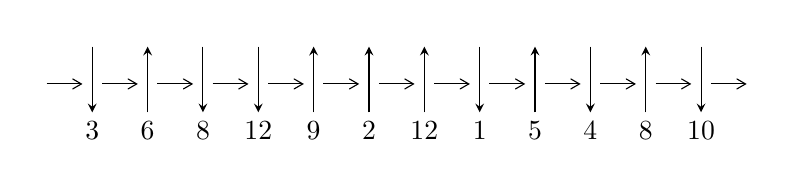
\begin{tikzpicture}[x=20pt, y=17pt]
	% nodes
	\node (C0) at (0, 0) {};
	\node (C1) at (1, 0) {};
	\node (C1U) at (1, +1) {};
	\node (C1D) at (1, -1) {3};

	\node (C2) at (2, 0) {};
	\node (C2U) at (2, +1) {};
	\node (C2D) at (2, -1) {6};

	\node (C3) at (3, 0) {};
	\node (C3U) at (3, +1) {};
	\node (C3D) at (3, -1) {8};

	\node (C4) at (4, 0) {};
	\node (C4U) at (4, +1) {};
	\node (C4D) at (4, -1) {12};

	\node (C5) at (5, 0) {};
	\node (C5U) at (5, +1) {};
	\node (C5D) at (5, -1) {9};

	\node (C6) at (6, 0) {};
	\node (C6U) at (6, +1) {};
	\node (C6D) at (6, -1) {2};

	\node (C7) at (7, 0) {};
	\node (C7U) at (7, +1) {};
	\node (C7D) at (7, -1) {12};

	\node (C8) at (8, 0) {};
	\node (C8U) at (8, +1) {};
	\node (C8D) at (8, -1) {1};

	\node (C9) at (9, 0) {};
	\node (C9U) at (9, +1) {};
	\node (C9D) at (9, -1) {5};

	\node (C10) at (10, 0) {};
	\node (C10U) at (10, +1) {};
	\node (C10D) at (10, -1) {4};

	\node (C11) at (11, 0) {};
	\node (C11U) at (11, +1) {};
	\node (C11D) at (11, -1) {8};

	\node (C12) at (12, 0) {};
	\node (C12U) at (12, +1) {};
	\node (C12D) at (12, -1) {10};
	\node (C13) at (13, 0) {};

	% arrows
	\draw[->,>={angle 60}]
	(C0) edge (C1) (C1) edge (C2) (C2) edge (C3) (C3) edge (C4) (C4) edge (C5) (C5) edge (C6) (C6) edge (C7) (C7) edge (C8) (C8) edge (C9) (C9) edge (C10) (C10) edge (C11) (C11) edge (C12) (C12) edge (C13) ;	\draw[->,>=stealth]
	(C1U) edge (C1D) (C2D) edge (C2U) (C3U) edge (C3D) (C4U) edge (C4D) (C5D) edge (C5U) (C6D) edge (C6U) (C7D) edge (C7U) (C8U) edge (C8D) (C9D) edge (C9U) (C10U) edge (C10D) (C11D) edge (C11U) (C12U) edge (C12D) ;
	\end{tikzpicture} \\
\hhline{~~} \\& 
\textbf{Solving Sequence} \\ \cline{2-2} 
 &
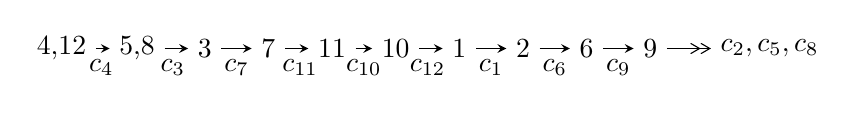
\begin{tikzpicture}[x=23pt, y=7pt]
	% node
	\node (A0) at (-1/8, 0) {4,12};
	\node (A1) at (17/16, 0) {5,8};
	\node (A2) at (17/8, 0) {3};
	\node (A3) at (25/8, 0) {7};
	\node (A4) at (33/8, 0) {11};
	\node (A5) at (41/8, 0) {10};
	\node (A6) at (49/8, 0) {1};
	\node (A7) at (57/8, 0) {2};
	\node (A8) at (65/8, 0) {6};
	\node (A9) at (73/8, 0) {9};
	\node (C1) at (1/2, -1) {$c_{4}$};
	\node (C2) at (13/8, -1) {$c_{3}$};
	\node (C3) at (21/8, -1) {$c_{7}$};
	\node (C4) at (29/8, -1) {$c_{11}$};
	\node (C5) at (37/8, -1) {$c_{10}$};
	\node (C6) at (45/8, -1) {$c_{12}$};
	\node (C7) at (53/8, -1) {$c_{1}$};
	\node (C8) at (61/8, -1) {$c_{6}$};
	\node (C9) at (69/8, -1) {$c_{9}$};
	\node (A10) at (11, 0) {$c_{2},c_{5},c_{8}$};

	% edge
	\draw[->,>=stealth]	
	(A0) edge (A1) (A1) edge (A2) (A2) edge (A3) (A3) edge (A4) (A4) edge (A5) (A5) edge (A6) (A6) edge (A7) (A7) edge (A8) (A8) edge (A9) ;
	\draw[->>,>={angle 60}]	
	(A9) edge (A10);
\end{tikzpicture} \\ 

\end{tabular} \\

\footnotetext{
The image of knot diagram is generated by the software ``\textbf{Draw programme}" developed by Andrew Bartholomew(\url{http://www.layer8.co.uk/maths/draw/index.htm\#Running-draw}), where we modified some parts for our purpose(\url{https://github.com/CATsTAILs/LinksPainter}).
}\phantom \\ \newline 
\centering \textbf{Ideals for irreducible components\footnotemark of $X_{\text{par}}$} 
 
\begin{align*}
I^u_{1}&=\langle 
3.28741\times10^{479} u^{73}-2.87933\times10^{478} u^{72}+\cdots+8.18620\times10^{484} b+8.77584\times10^{484},\\
\phantom{I^u_{1}}&\phantom{= \langle  }-9.92062\times10^{484} u^{73}-8.13255\times10^{483} u^{72}+\cdots+1.40884\times10^{490} a-5.50149\times10^{490},\\
\phantom{I^u_{1}}&\phantom{= \langle  }u^{74}+17 u^{72}+\cdots+566418 u+172099\rangle \\
I^u_{2}&=\langle 
3.09881\times10^{32} u^{23}-1.01801\times10^{33} u^{22}+\cdots+2.58026\times10^{32} b+5.97065\times10^{32},\\
\phantom{I^u_{2}}&\phantom{= \langle  }-9.65284\times10^{32} u^{23}+3.27534\times10^{33} u^{22}+\cdots+2.58026\times10^{32} a-2.48109\times10^{33},\;u^{24}-3 u^{23}+\cdots+3 u+1\rangle \\
\\
\end{align*}
\raggedright * 2 irreducible components of $\dim_{\mathbb{C}}=0$, with total 98 representations.\\
\footnotetext{All coefficients of polynomials are rational numbers. But the coefficients are sometimes approximated in decimal forms when there is not enough margin.}
\newpage
\renewcommand{\arraystretch}{1}
\centering \section*{I. $I^u_{1}= \langle 3.29\times10^{479} u^{73}-2.88\times10^{478} u^{72}+\cdots+8.19\times10^{484} b+8.78\times10^{484},\;-9.92\times10^{484} u^{73}-8.13\times10^{483} u^{72}+\cdots+1.41\times10^{490} a-5.50\times10^{490},\;u^{74}+17 u^{72}+\cdots+566418 u+172099 \rangle$}
\flushleft \textbf{(i) Arc colorings}\\
\begin{tabular}{m{7pt} m{180pt} m{7pt} m{180pt} }
\flushright $a_{4}=$&$\begin{pmatrix}1\\0\end{pmatrix}$ \\
\flushright $a_{12}=$&$\begin{pmatrix}0\\u\end{pmatrix}$ \\
\flushright $a_{5}=$&$\begin{pmatrix}1\\u^2\end{pmatrix}$ \\
\flushright $a_{8}=$&$\begin{pmatrix}7.04171\times10^{-6} u^{73}+5.77253\times10^{-7} u^{72}+\cdots+22.2661 u+3.90499\\-4.01579\times10^{-6} u^{73}+3.51729\times10^{-7} u^{72}+\cdots-12.7786 u-1.07203\end{pmatrix}$ \\
\flushright $a_{3}=$&$\begin{pmatrix}4.10227\times10^{-6} u^{73}-5.68165\times10^{-7} u^{72}+\cdots+9.97933 u-6.12982\\2.46937\times10^{-6} u^{73}-9.40460\times10^{-7} u^{72}+\cdots+3.33975 u+4.81554\end{pmatrix}$ \\
\flushright $a_{7}=$&$\begin{pmatrix}7.04171\times10^{-6} u^{73}+5.77253\times10^{-7} u^{72}+\cdots+22.2661 u+3.90499\\-5.02310\times10^{-6} u^{73}+9.02842\times10^{-7} u^{72}+\cdots-14.3175 u-1.17137\end{pmatrix}$ \\
\flushright $a_{11}=$&$\begin{pmatrix}3.03522\times10^{-6} u^{73}-5.96192\times10^{-7} u^{72}+\cdots+17.7584 u+3.27815\\-5.68165\times10^{-7} u^{73}+4.05095\times10^{-7} u^{72}+\cdots-8.45342 u-0.705996\end{pmatrix}$ \\
\flushright $a_{10}=$&$\begin{pmatrix}2.46706\times10^{-6} u^{73}-1.91097\times10^{-7} u^{72}+\cdots+9.30498 u+2.57215\\-5.68165\times10^{-7} u^{73}+4.05095\times10^{-7} u^{72}+\cdots-8.45342 u-0.705996\end{pmatrix}$ \\
\flushright $a_{1}=$&$\begin{pmatrix}-3.83456\times10^{-6} u^{73}+2.72856\times10^{-6} u^{72}+\cdots+1.24718 u+1.08281\\9.25604\times10^{-8} u^{73}-1.11084\times10^{-8} u^{72}+\cdots-3.16667 u-1.19214\end{pmatrix}$ \\
\flushright $a_{2}=$&$\begin{pmatrix}-0.0000145703 u^{73}+3.10645\times10^{-6} u^{72}+\cdots-21.8387 u+2.58100\\7.25950\times10^{-6} u^{73}-1.35849\times10^{-6} u^{72}+\cdots+7.69972 u-4.14218\end{pmatrix}$ \\
\flushright $a_{6}=$&$\begin{pmatrix}3.33389\times10^{-6} u^{73}+1.49484\times10^{-6} u^{72}+\cdots+15.6618 u-1.68488\\2.06380\times10^{-6} u^{73}-3.06763\times10^{-6} u^{72}+\cdots-4.88783 u+1.52464\end{pmatrix}$ \\
\flushright $a_{9}=$&$\begin{pmatrix}3.64252\times10^{-6} u^{73}-7.63769\times10^{-7} u^{72}+\cdots+17.4421 u+3.31103\\-7.64708\times10^{-8} u^{73}+8.94112\times10^{-7} u^{72}+\cdots-8.33134 u-0.607440\end{pmatrix}$\\&\end{tabular}
\flushleft \textbf{(ii) Obstruction class $= -1$}\\~\\
\flushleft \textbf{(iii) Cusp Shapes $= -0.0000403389 u^{73}+0.0000203868 u^{72}+\cdots-47.2240 u+0.0222812$}\\~\\
\newpage\renewcommand{\arraystretch}{1}
\flushleft \textbf{(iv) u-Polynomials at the component}\newline \\
\begin{tabular}{m{50pt}|m{274pt}}
Crossings & \hspace{64pt}u-Polynomials at each crossing \\
\hline $$\begin{aligned}c_{1}\end{aligned}$$&$\begin{aligned}
&u^{74}+34 u^{73}+\cdots+340368 u+13456
\end{aligned}$\\
\hline $$\begin{aligned}c_{2},c_{6}\end{aligned}$$&$\begin{aligned}
&u^{74}-2 u^{73}+\cdots-192 u+116
\end{aligned}$\\
\hline $$\begin{aligned}c_{3}\end{aligned}$$&$\begin{aligned}
&u^{74}-3 u^{73}+\cdots+2408 u+184
\end{aligned}$\\
\hline $$\begin{aligned}c_{4}\end{aligned}$$&$\begin{aligned}
&u^{74}+17 u^{72}+\cdots-566418 u+172099
\end{aligned}$\\
\hline $$\begin{aligned}c_{5},c_{9}\end{aligned}$$&$\begin{aligned}
&u^{74}-4 u^{73}+\cdots-69 u+131
\end{aligned}$\\
\hline $$\begin{aligned}c_{7},c_{11}\end{aligned}$$&$\begin{aligned}
&u^{74}- u^{73}+\cdots-325282 u+19639
\end{aligned}$\\
\hline $$\begin{aligned}c_{8}\end{aligned}$$&$\begin{aligned}
&u^{74}+3 u^{73}+\cdots-8536 u+1093
\end{aligned}$\\
\hline $$\begin{aligned}c_{10}\end{aligned}$$&$\begin{aligned}
&u^{74}-2 u^{73}+\cdots+49021 u+18569
\end{aligned}$\\
\hline $$\begin{aligned}c_{12}\end{aligned}$$&$\begin{aligned}
&u^{74}-9 u^{73}+\cdots-22 u+1
\end{aligned}$\\
\hline
\end{tabular}\\~\\
\newpage\renewcommand{\arraystretch}{1}
\flushleft \textbf{(v) Riley Polynomials at the component}\newline \\
\begin{tabular}{m{50pt}|m{274pt}}
Crossings & \hspace{64pt}Riley Polynomials at each crossing \\
\hline $$\begin{aligned}c_{1}\end{aligned}$$&$\begin{aligned}
&y^{74}+26 y^{73}+\cdots+2544232064 y+181063936
\end{aligned}$\\
\hline $$\begin{aligned}c_{2},c_{6}\end{aligned}$$&$\begin{aligned}
&y^{74}+34 y^{73}+\cdots+340368 y+13456
\end{aligned}$\\
\hline $$\begin{aligned}c_{3}\end{aligned}$$&$\begin{aligned}
&y^{74}+103 y^{73}+\cdots+155040 y+33856
\end{aligned}$\\
\hline $$\begin{aligned}c_{4}\end{aligned}$$&$\begin{aligned}
&y^{74}+34 y^{73}+\cdots+998146334424 y+29618065801
\end{aligned}$\\
\hline $$\begin{aligned}c_{5},c_{9}\end{aligned}$$&$\begin{aligned}
&y^{74}+44 y^{73}+\cdots+371471 y+17161
\end{aligned}$\\
\hline $$\begin{aligned}c_{7},c_{11}\end{aligned}$$&$\begin{aligned}
&y^{74}-93 y^{73}+\cdots-43352903060 y+385690321
\end{aligned}$\\
\hline $$\begin{aligned}c_{8}\end{aligned}$$&$\begin{aligned}
&y^{74}+9 y^{73}+\cdots+23967760 y+1194649
\end{aligned}$\\
\hline $$\begin{aligned}c_{10}\end{aligned}$$&$\begin{aligned}
&y^{74}+90 y^{73}+\cdots+2650383495 y+344807761
\end{aligned}$\\
\hline $$\begin{aligned}c_{12}\end{aligned}$$&$\begin{aligned}
&y^{74}-3 y^{73}+\cdots-56 y^2+1
\end{aligned}$\\
\hline
\end{tabular}\\~\\
\newpage\flushleft \textbf{(vi) Complex Volumes and Cusp Shapes}
$$\begin{array}{c|c|c}  
\text{Solutions to }I^u_{1}& \I (\text{vol} + \sqrt{-1}CS) & \text{Cusp shape}\\
 \hline 
\begin{aligned}
u &= \phantom{-}0.934779 + 0.503629 I \\
a &= -1.194160 - 0.295302 I \\
b &= -0.254337 - 0.211732 I\end{aligned}
 & -0.307331 - 1.010300 I & \phantom{-0.000000 } 0 \\ \hline\begin{aligned}
u &= \phantom{-}0.934779 - 0.503629 I \\
a &= -1.194160 + 0.295302 I \\
b &= -0.254337 + 0.211732 I\end{aligned}
 & -0.307331 + 1.010300 I & \phantom{-0.000000 } 0 \\ \hline\begin{aligned}
u &= -1.002250 + 0.372992 I \\
a &= -0.268943 - 0.748372 I \\
b &= \phantom{-}0.369189 + 0.429283 I\end{aligned}
 & -6.55930 + 3.70588 I & -5.57212 + 0. I\phantom{ +0.000000I} \\ \hline\begin{aligned}
u &= -1.002250 - 0.372992 I \\
a &= -0.268943 + 0.748372 I \\
b &= \phantom{-}0.369189 - 0.429283 I\end{aligned}
 & -6.55930 - 3.70588 I & -5.57212 + 0. I\phantom{ +0.000000I} \\ \hline\begin{aligned}
u &= -0.374952 + 0.843157 I \\
a &= -0.597418 - 0.434941 I \\
b &= -1.021630 - 0.003737 I\end{aligned}
 & -5.47234 + 0.86790 I & -3.59499 + 0.79812 I \\ \hline\begin{aligned}
u &= -0.374952 - 0.843157 I \\
a &= -0.597418 + 0.434941 I \\
b &= -1.021630 + 0.003737 I\end{aligned}
 & -5.47234 - 0.86790 I & -3.59499 - 0.79812 I \\ \hline\begin{aligned}
u &= \phantom{-}1.082250 + 0.107771 I \\
a &= -0.608665 + 0.566681 I \\
b &= -0.859754 - 0.446277 I\end{aligned}
 & -0.94736 - 5.88404 I & \phantom{-0.000000 -}0. + 8.12047 I \\ \hline\begin{aligned}
u &= \phantom{-}1.082250 - 0.107771 I \\
a &= -0.608665 - 0.566681 I \\
b &= -0.859754 + 0.446277 I\end{aligned}
 & -0.94736 + 5.88404 I & \phantom{-0.000000 } 0. - 8.12047 I \\ \hline\begin{aligned}
u &= -0.435194 + 0.774098 I \\
a &= \phantom{-}1.52616 + 0.04105 I \\
b &= \phantom{-}0.110382 - 0.125676 I\end{aligned}
 & \phantom{-}0.58998 - 3.66458 I & \phantom{-}2.57268 + 0.26922 I \\ \hline\begin{aligned}
u &= -0.435194 - 0.774098 I \\
a &= \phantom{-}1.52616 - 0.04105 I \\
b &= \phantom{-}0.110382 + 0.125676 I\end{aligned}
 & \phantom{-}0.58998 + 3.66458 I & \phantom{-}2.57268 - 0.26922 I\\
 \hline 
 \end{array}$$\newpage$$\begin{array}{c|c|c}  
\text{Solutions to }I^u_{1}& \I (\text{vol} + \sqrt{-1}CS) & \text{Cusp shape}\\
 \hline 
\begin{aligned}
u &= -0.810830 + 0.337697 I \\
a &= \phantom{-}0.464928 + 0.856520 I \\
b &= \phantom{-}0.242275 - 0.682677 I\end{aligned}
 & \phantom{-}1.26684 + 1.82853 I & \phantom{-}1.78603 - 4.52891 I \\ \hline\begin{aligned}
u &= -0.810830 - 0.337697 I \\
a &= \phantom{-}0.464928 - 0.856520 I \\
b &= \phantom{-}0.242275 + 0.682677 I\end{aligned}
 & \phantom{-}1.26684 - 1.82853 I & \phantom{-}1.78603 + 4.52891 I \\ \hline\begin{aligned}
u &= -0.016733 + 0.853800 I \\
a &= -0.61995 - 2.02125 I \\
b &= -0.15930 + 1.56017 I\end{aligned}
 & \phantom{-}8.24996 - 1.54945 I & \phantom{-}3.85987 + 1.93387 I \\ \hline\begin{aligned}
u &= -0.016733 - 0.853800 I \\
a &= -0.61995 + 2.02125 I \\
b &= -0.15930 - 1.56017 I\end{aligned}
 & \phantom{-}8.24996 + 1.54945 I & \phantom{-}3.85987 - 1.93387 I \\ \hline\begin{aligned}
u &= \phantom{-}0.639477 + 0.519628 I \\
a &= \phantom{-}0.565407 + 0.564947 I \\
b &= \phantom{-}0.207804 - 0.033918 I\end{aligned}
 & -1.11297 - 1.12209 I & -5.31504 + 3.79418 I \\ \hline\begin{aligned}
u &= \phantom{-}0.639477 - 0.519628 I \\
a &= \phantom{-}0.565407 - 0.564947 I \\
b &= \phantom{-}0.207804 + 0.033918 I\end{aligned}
 & -1.11297 + 1.12209 I & -5.31504 - 3.79418 I \\ \hline\begin{aligned}
u &= -0.350425 + 0.723346 I \\
a &= \phantom{-}0.370401 - 0.209665 I \\
b &= \phantom{-}0.115118 + 0.975558 I\end{aligned}
 & \phantom{-}0.72481 - 1.83639 I & \phantom{-}1.12069 + 4.87359 I \\ \hline\begin{aligned}
u &= -0.350425 - 0.723346 I \\
a &= \phantom{-}0.370401 + 0.209665 I \\
b &= \phantom{-}0.115118 - 0.975558 I\end{aligned}
 & \phantom{-}0.72481 + 1.83639 I & \phantom{-}1.12069 - 4.87359 I \\ \hline\begin{aligned}
u &= \phantom{-}0.457795 + 0.617756 I \\
a &= \phantom{-}1.43093 - 1.15085 I \\
b &= \phantom{-}0.47311 + 1.48482 I\end{aligned}
 & \phantom{-}2.48087 - 3.10809 I & \phantom{-}2.96786 + 1.73580 I \\ \hline\begin{aligned}
u &= \phantom{-}0.457795 - 0.617756 I \\
a &= \phantom{-}1.43093 + 1.15085 I \\
b &= \phantom{-}0.47311 - 1.48482 I\end{aligned}
 & \phantom{-}2.48087 + 3.10809 I & \phantom{-}2.96786 - 1.73580 I\\
 \hline 
 \end{array}$$\newpage$$\begin{array}{c|c|c}  
\text{Solutions to }I^u_{1}& \I (\text{vol} + \sqrt{-1}CS) & \text{Cusp shape}\\
 \hline 
\begin{aligned}
u &= -0.216764 + 0.727146 I \\
a &= \phantom{-}0.14023 - 2.38086 I \\
b &= \phantom{-}0.02763 + 1.51400 I\end{aligned}
 & \phantom{-}5.47332 + 8.05912 I & \phantom{-}0.18543 - 6.05650 I \\ \hline\begin{aligned}
u &= -0.216764 - 0.727146 I \\
a &= \phantom{-}0.14023 + 2.38086 I \\
b &= \phantom{-}0.02763 - 1.51400 I\end{aligned}
 & \phantom{-}5.47332 - 8.05912 I & \phantom{-}0.18543 + 6.05650 I \\ \hline\begin{aligned}
u &= \phantom{-}0.319181 + 1.202940 I \\
a &= \phantom{-}0.431572 - 0.366985 I \\
b &= \phantom{-}1.203360 + 0.711683 I\end{aligned}
 & -0.85478 - 3.82352 I & \phantom{-0.000000 } 0 \\ \hline\begin{aligned}
u &= \phantom{-}0.319181 - 1.202940 I \\
a &= \phantom{-}0.431572 + 0.366985 I \\
b &= \phantom{-}1.203360 - 0.711683 I\end{aligned}
 & -0.85478 + 3.82352 I & \phantom{-0.000000 } 0 \\ \hline\begin{aligned}
u &= -0.467790 + 0.563021 I \\
a &= \phantom{-}0.549943 + 1.084810 I \\
b &= -0.532295 - 1.238560 I\end{aligned}
 & \phantom{-}1.58966 + 1.29211 I & \phantom{-}4.03888 + 5.21852 I \\ \hline\begin{aligned}
u &= -0.467790 - 0.563021 I \\
a &= \phantom{-}0.549943 - 1.084810 I \\
b &= -0.532295 + 1.238560 I\end{aligned}
 & \phantom{-}1.58966 - 1.29211 I & \phantom{-}4.03888 - 5.21852 I \\ \hline\begin{aligned}
u &= -0.547174 + 0.464224 I \\
a &= -1.47110 + 1.20328 I \\
b &= -0.093733 + 0.616829 I\end{aligned}
 & -9.47431 + 0.30033 I & -4.15634 + 8.16557 I \\ \hline\begin{aligned}
u &= -0.547174 - 0.464224 I \\
a &= -1.47110 - 1.20328 I \\
b &= -0.093733 - 0.616829 I\end{aligned}
 & -9.47431 - 0.30033 I & -4.15634 - 8.16557 I \\ \hline\begin{aligned}
u &= \phantom{-}1.088520 + 0.716063 I \\
a &= \phantom{-}0.709402 + 0.222922 I \\
b &= -0.110085 + 0.256217 I\end{aligned}
 & -1.25400 - 2.51544 I & \phantom{-0.000000 } 0 \\ \hline\begin{aligned}
u &= \phantom{-}1.088520 - 0.716063 I \\
a &= \phantom{-}0.709402 - 0.222922 I \\
b &= -0.110085 - 0.256217 I\end{aligned}
 & -1.25400 + 2.51544 I & \phantom{-0.000000 } 0\\
 \hline 
 \end{array}$$\newpage$$\begin{array}{c|c|c}  
\text{Solutions to }I^u_{1}& \I (\text{vol} + \sqrt{-1}CS) & \text{Cusp shape}\\
 \hline 
\begin{aligned}
u &= -0.518744 + 1.213760 I \\
a &= -0.419984 - 0.307566 I \\
b &= -1.64440 + 0.69687 I\end{aligned}
 & -3.28433 + 8.86378 I & \phantom{-0.000000 } 0 \\ \hline\begin{aligned}
u &= -0.518744 - 1.213760 I \\
a &= -0.419984 + 0.307566 I \\
b &= -1.64440 - 0.69687 I\end{aligned}
 & -3.28433 - 8.86378 I & \phantom{-0.000000 } 0 \\ \hline\begin{aligned}
u &= \phantom{-}0.512571 + 0.438202 I \\
a &= -0.691080 - 0.061151 I \\
b &= \phantom{-}1.050440 - 0.405546 I\end{aligned}
 & \phantom{-}0.61911 + 3.11056 I & \phantom{-}3.75248 + 0.56298 I \\ \hline\begin{aligned}
u &= \phantom{-}0.512571 - 0.438202 I \\
a &= -0.691080 + 0.061151 I \\
b &= \phantom{-}1.050440 + 0.405546 I\end{aligned}
 & \phantom{-}0.61911 - 3.11056 I & \phantom{-}3.75248 - 0.56298 I \\ \hline\begin{aligned}
u &= -0.521401 + 0.376721 I \\
a &= \phantom{-}1.142470 + 0.548301 I \\
b &= -1.154480 - 0.714467 I\end{aligned}
 & \phantom{-}1.65020 + 1.37390 I & \phantom{-}18.4680 - 12.7347 I \\ \hline\begin{aligned}
u &= -0.521401 - 0.376721 I \\
a &= \phantom{-}1.142470 - 0.548301 I \\
b &= -1.154480 + 0.714467 I\end{aligned}
 & \phantom{-}1.65020 - 1.37390 I & \phantom{-}18.4680 + 12.7347 I \\ \hline\begin{aligned}
u &= \phantom{-}0.329499 + 0.490134 I \\
a &= -0.151663 + 0.089033 I \\
b &= \phantom{-}0.744003 + 0.776343 I\end{aligned}
 & -0.25653 - 2.28963 I & -1.31647 + 4.44383 I \\ \hline\begin{aligned}
u &= \phantom{-}0.329499 - 0.490134 I \\
a &= -0.151663 - 0.089033 I \\
b &= \phantom{-}0.744003 - 0.776343 I\end{aligned}
 & -0.25653 + 2.28963 I & -1.31647 - 4.44383 I \\ \hline\begin{aligned}
u &= -1.29609 + 0.63868 I \\
a &= -0.714241 + 0.014858 I \\
b &= \phantom{-}0.224602 + 0.245414 I\end{aligned}
 & -2.18586 + 8.15624 I & \phantom{-0.000000 } 0 \\ \hline\begin{aligned}
u &= -1.29609 - 0.63868 I \\
a &= -0.714241 - 0.014858 I \\
b &= \phantom{-}0.224602 - 0.245414 I\end{aligned}
 & -2.18586 - 8.15624 I & \phantom{-0.000000 } 0\\
 \hline 
 \end{array}$$\newpage$$\begin{array}{c|c|c}  
\text{Solutions to }I^u_{1}& \I (\text{vol} + \sqrt{-1}CS) & \text{Cusp shape}\\
 \hline 
\begin{aligned}
u &= -0.57675 + 1.33502 I \\
a &= -0.419449 - 1.215320 I \\
b &= -0.31506 + 1.85613 I\end{aligned}
 & \phantom{-}10.81600 + 3.74825 I & \phantom{-0.000000 } 0 \\ \hline\begin{aligned}
u &= -0.57675 - 1.33502 I \\
a &= -0.419449 + 1.215320 I \\
b &= -0.31506 - 1.85613 I\end{aligned}
 & \phantom{-}10.81600 - 3.74825 I & \phantom{-0.000000 } 0 \\ \hline\begin{aligned}
u &= \phantom{-}0.071209 + 0.532949 I \\
a &= -0.12914 + 2.57050 I \\
b &= -0.01065 - 2.13563 I\end{aligned}
 & \phantom{-}2.73609 - 2.38466 I & -10.42559 + 0.76440 I \\ \hline\begin{aligned}
u &= \phantom{-}0.071209 - 0.532949 I \\
a &= -0.12914 - 2.57050 I \\
b &= -0.01065 + 2.13563 I\end{aligned}
 & \phantom{-}2.73609 + 2.38466 I & -10.42559 - 0.76440 I \\ \hline\begin{aligned}
u &= \phantom{-}1.27357 + 0.72807 I \\
a &= -0.414781 - 0.349604 I \\
b &= -0.275822 + 0.512285 I\end{aligned}
 & -6.32359 - 3.97690 I & \phantom{-0.000000 } 0 \\ \hline\begin{aligned}
u &= \phantom{-}1.27357 - 0.72807 I \\
a &= -0.414781 + 0.349604 I \\
b &= -0.275822 - 0.512285 I\end{aligned}
 & -6.32359 + 3.97690 I & \phantom{-0.000000 } 0 \\ \hline\begin{aligned}
u &= \phantom{-}0.12017 + 1.51738 I \\
a &= \phantom{-}1.011970 - 0.315727 I \\
b &= \phantom{-}0.379110 + 0.559913 I\end{aligned}
 & -0.39783 + 1.72887 I & \phantom{-0.000000 } 0 \\ \hline\begin{aligned}
u &= \phantom{-}0.12017 - 1.51738 I \\
a &= \phantom{-}1.011970 + 0.315727 I \\
b &= \phantom{-}0.379110 - 0.559913 I\end{aligned}
 & -0.39783 - 1.72887 I & \phantom{-0.000000 } 0 \\ \hline\begin{aligned}
u &= \phantom{-}0.71828 + 1.39939 I \\
a &= \phantom{-}0.343326 - 1.136520 I \\
b &= \phantom{-}0.33207 + 1.92509 I\end{aligned}
 & \phantom{-}9.56306 - 9.81975 I & \phantom{-0.000000 } 0 \\ \hline\begin{aligned}
u &= \phantom{-}0.71828 - 1.39939 I \\
a &= \phantom{-}0.343326 + 1.136520 I \\
b &= \phantom{-}0.33207 - 1.92509 I\end{aligned}
 & \phantom{-}9.56306 + 9.81975 I & \phantom{-0.000000 } 0\\
 \hline 
 \end{array}$$\newpage$$\begin{array}{c|c|c}  
\text{Solutions to }I^u_{1}& \I (\text{vol} + \sqrt{-1}CS) & \text{Cusp shape}\\
 \hline 
\begin{aligned}
u &= \phantom{-}0.97511 + 1.28716 I \\
a &= -0.633764 + 1.006090 I \\
b &= -0.40476 - 1.67994 I\end{aligned}
 & \phantom{-}0.54467 - 6.58007 I & \phantom{-0.000000 } 0 \\ \hline\begin{aligned}
u &= \phantom{-}0.97511 - 1.28716 I \\
a &= -0.633764 - 1.006090 I \\
b &= -0.40476 + 1.67994 I\end{aligned}
 & \phantom{-}0.54467 + 6.58007 I & \phantom{-0.000000 } 0 \\ \hline\begin{aligned}
u &= -0.101175 + 0.268318 I \\
a &= \phantom{-}1.32347 + 2.96824 I \\
b &= \phantom{-}0.00255 - 1.97774 I\end{aligned}
 & \phantom{-}1.15369 + 1.33003 I & \phantom{-}0.26910 - 8.47917 I \\ \hline\begin{aligned}
u &= -0.101175 - 0.268318 I \\
a &= \phantom{-}1.32347 - 2.96824 I \\
b &= \phantom{-}0.00255 + 1.97774 I\end{aligned}
 & \phantom{-}1.15369 - 1.33003 I & \phantom{-}0.26910 + 8.47917 I \\ \hline\begin{aligned}
u &= \phantom{-}1.33047 + 1.16519 I \\
a &= \phantom{-}0.478417 - 0.613747 I \\
b &= \phantom{-}0.66765 + 1.86705 I\end{aligned}
 & \phantom{-}3.05422 - 4.02557 I & \phantom{-0.000000 } 0 \\ \hline\begin{aligned}
u &= \phantom{-}1.33047 - 1.16519 I \\
a &= \phantom{-}0.478417 + 0.613747 I \\
b &= \phantom{-}0.66765 - 1.86705 I\end{aligned}
 & \phantom{-}3.05422 + 4.02557 I & \phantom{-0.000000 } 0 \\ \hline\begin{aligned}
u &= \phantom{-}0.42249 + 1.74075 I \\
a &= -0.871746 - 0.415011 I \\
b &= -0.361054 + 0.602089 I\end{aligned}
 & -1.16452 - 7.75367 I & \phantom{-0.000000 } 0 \\ \hline\begin{aligned}
u &= \phantom{-}0.42249 - 1.74075 I \\
a &= -0.871746 + 0.415011 I \\
b &= -0.361054 - 0.602089 I\end{aligned}
 & -1.16452 + 7.75367 I & \phantom{-0.000000 } 0 \\ \hline\begin{aligned}
u &= -0.42488 + 1.77560 I \\
a &= \phantom{-}0.300223 + 1.183900 I \\
b &= \phantom{-}0.14185 - 1.70906 I\end{aligned}
 & \phantom{-}9.45918 + 3.10998 I & \phantom{-0.000000 } 0 \\ \hline\begin{aligned}
u &= -0.42488 - 1.77560 I \\
a &= \phantom{-}0.300223 - 1.183900 I \\
b &= \phantom{-}0.14185 + 1.70906 I\end{aligned}
 & \phantom{-}9.45918 - 3.10998 I & \phantom{-0.000000 } 0\\
 \hline 
 \end{array}$$\newpage$$\begin{array}{c|c|c}  
\text{Solutions to }I^u_{1}& \I (\text{vol} + \sqrt{-1}CS) & \text{Cusp shape}\\
 \hline 
\begin{aligned}
u &= \phantom{-}0.07853 + 1.91814 I \\
a &= -0.171569 + 1.111140 I \\
b &= -0.07595 - 1.74382 I\end{aligned}
 & \phantom{-}8.50999 + 3.70014 I & \phantom{-0.000000 } 0 \\ \hline\begin{aligned}
u &= \phantom{-}0.07853 - 1.91814 I \\
a &= -0.171569 - 1.111140 I \\
b &= -0.07595 + 1.74382 I\end{aligned}
 & \phantom{-}8.50999 - 3.70014 I & \phantom{-0.000000 } 0 \\ \hline\begin{aligned}
u &= -1.84596 + 0.63181 I \\
a &= -0.469448 - 0.493054 I \\
b &= -0.62297 + 1.95623 I\end{aligned}
 & \phantom{-}3.44928 + 1.73681 I & \phantom{-0.000000 } 0 \\ \hline\begin{aligned}
u &= -1.84596 - 0.63181 I \\
a &= -0.469448 + 0.493054 I \\
b &= -0.62297 - 1.95623 I\end{aligned}
 & \phantom{-}3.44928 - 1.73681 I & \phantom{-0.000000 } 0 \\ \hline\begin{aligned}
u &= -1.32220 + 1.55486 I \\
a &= \phantom{-}0.440807 + 0.919591 I \\
b &= \phantom{-}0.35456 - 1.87560 I\end{aligned}
 & \phantom{-}8.07490 + 10.29220 I & \phantom{-0.000000 } 0 \\ \hline\begin{aligned}
u &= -1.32220 - 1.55486 I \\
a &= \phantom{-}0.440807 - 0.919591 I \\
b &= \phantom{-}0.35456 + 1.87560 I\end{aligned}
 & \phantom{-}8.07490 - 10.29220 I & \phantom{-0.000000 } 0 \\ \hline\begin{aligned}
u &= \phantom{-}1.48295 + 1.47987 I \\
a &= -0.415885 + 0.867026 I \\
b &= -0.38217 - 1.94494 I\end{aligned}
 & \phantom{-}5.8809 - 16.7307 I & \phantom{-0.000000 } 0 \\ \hline\begin{aligned}
u &= \phantom{-}1.48295 - 1.47987 I \\
a &= -0.415885 - 0.867026 I \\
b &= -0.38217 + 1.94494 I\end{aligned}
 & \phantom{-}5.8809 + 16.7307 I & \phantom{-0.000000 } 0 \\ \hline\begin{aligned}
u &= \phantom{-}2.27181 + 1.64904 I \\
a &= \phantom{-}0.460402 - 0.548295 I \\
b &= \phantom{-}0.54956 + 1.75108 I\end{aligned}
 & \phantom{-}5.60799 - 0.31469 I & \phantom{-0.000000 } 0 \\ \hline\begin{aligned}
u &= \phantom{-}2.27181 - 1.64904 I \\
a &= \phantom{-}0.460402 + 0.548295 I \\
b &= \phantom{-}0.54956 - 1.75108 I\end{aligned}
 & \phantom{-}5.60799 + 0.31469 I & \phantom{-0.000000 } 0\\
 \hline 
 \end{array}$$\newpage$$\begin{array}{c|c|c}  
\text{Solutions to }I^u_{1}& \I (\text{vol} + \sqrt{-1}CS) & \text{Cusp shape}\\
 \hline 
\begin{aligned}
u &= -2.49665 + 1.28593 I \\
a &= -0.451579 - 0.553382 I \\
b &= -0.50037 + 1.80564 I\end{aligned}
 & \phantom{-}5.54289 + 5.38790 I & \phantom{-0.000000 } 0 \\ \hline\begin{aligned}
u &= -2.49665 - 1.28593 I \\
a &= -0.451579 + 0.553382 I \\
b &= -0.50037 - 1.80564 I\end{aligned}
 & \phantom{-}5.54289 - 5.38790 I & \phantom{-0.000000 } 0 \\ \hline\begin{aligned}
u &= -0.78268 + 3.57446 I \\
a &= \phantom{-}0.064497 + 0.693383 I \\
b &= \phantom{-}0.08356 - 2.09334 I\end{aligned}
 & \phantom{-}8.35485 + 3.17981 I & \phantom{-0.000000 } 0 \\ \hline\begin{aligned}
u &= -0.78268 - 3.57446 I \\
a &= \phantom{-}0.064497 - 0.693383 I \\
b &= \phantom{-}0.08356 + 2.09334 I\end{aligned}
 & \phantom{-}8.35485 - 3.17981 I & \phantom{-0.000000 } 0\\
 \hline 
 \end{array}$$\newpage\newpage\renewcommand{\arraystretch}{1}
\centering \section*{II. $I^u_{2}= \langle 3.10\times10^{32} u^{23}-1.02\times10^{33} u^{22}+\cdots+2.58\times10^{32} b+5.97\times10^{32},\;-9.65\times10^{32} u^{23}+3.28\times10^{33} u^{22}+\cdots+2.58\times10^{32} a-2.48\times10^{33},\;u^{24}-3 u^{23}+\cdots+3 u+1 \rangle$}
\flushleft \textbf{(i) Arc colorings}\\
\begin{tabular}{m{7pt} m{180pt} m{7pt} m{180pt} }
\flushright $a_{4}=$&$\begin{pmatrix}1\\0\end{pmatrix}$ \\
\flushright $a_{12}=$&$\begin{pmatrix}0\\u\end{pmatrix}$ \\
\flushright $a_{5}=$&$\begin{pmatrix}1\\u^2\end{pmatrix}$ \\
\flushright $a_{8}=$&$\begin{pmatrix}3.74103 u^{23}-12.6938 u^{22}+\cdots+10.1999 u+9.61566\\-1.20097 u^{23}+3.94538 u^{22}+\cdots-4.41854 u-2.31397\end{pmatrix}$ \\
\flushright $a_{3}=$&$\begin{pmatrix}-0.905445 u^{23}+3.08921 u^{22}+\cdots-1.58493 u-3.29115\\0.744548 u^{23}-2.26904 u^{22}+\cdots+3.33781 u+3.02014\end{pmatrix}$ \\
\flushright $a_{7}=$&$\begin{pmatrix}3.74103 u^{23}-12.6938 u^{22}+\cdots+10.1999 u+9.61566\\-0.495914 u^{23}+1.56323 u^{22}+\cdots-3.74734 u-0.843228\end{pmatrix}$ \\
\flushright $a_{11}=$&$\begin{pmatrix}2.50091 u^{23}-8.64542 u^{22}+\cdots+4.71165 u+5.73810\\0.372873 u^{23}-1.41387 u^{22}+\cdots-0.574815 u+0.905445\end{pmatrix}$ \\
\flushright $a_{10}=$&$\begin{pmatrix}2.87378 u^{23}-10.0593 u^{22}+\cdots+4.13684 u+6.64354\\0.372873 u^{23}-1.41387 u^{22}+\cdots-0.574815 u+0.905445\end{pmatrix}$ \\
\flushright $a_{1}=$&$\begin{pmatrix}-3.28358 u^{23}+11.2247 u^{22}+\cdots-4.93024 u-7.38504\\-0.132750 u^{23}+0.365444 u^{22}+\cdots+1.06308 u-0.0278847\end{pmatrix}$ \\
\flushright $a_{2}=$&$\begin{pmatrix}-3.04569 u^{23}+10.5278 u^{22}+\cdots-5.14348 u-8.23501\\0.415551 u^{23}-1.42417 u^{22}+\cdots+2.99968 u+2.58734\end{pmatrix}$ \\
\flushright $a_{6}=$&$\begin{pmatrix}-1.13356 u^{23}+3.73009 u^{22}+\cdots-1.83336 u-2.03684\\-0.561956 u^{23}+2.08239 u^{22}+\cdots-0.145765 u-0.429411\end{pmatrix}$ \\
\flushright $a_{9}=$&$\begin{pmatrix}3.15671 u^{23}-10.9173 u^{22}+\cdots+6.15169 u+7.17604\\0.289587 u^{23}-1.13640 u^{22}+\cdots-0.830127 u+0.914649\end{pmatrix}$\\&\end{tabular}
\flushleft \textbf{(ii) Obstruction class $= 1$}\\~\\
\flushleft \textbf{(iii) Cusp Shapes $= -19.3109 u^{23}+64.5263 u^{22}+\cdots-45.8349 u-32.8279$}\\~\\
\newpage\renewcommand{\arraystretch}{1}
\flushleft \textbf{(iv) u-Polynomials at the component}\newline \\
\begin{tabular}{m{50pt}|m{274pt}}
Crossings & \hspace{64pt}u-Polynomials at each crossing \\
\hline $$\begin{aligned}c_{1}\end{aligned}$$&$\begin{aligned}
&u^{24}-17 u^{23}+\cdots-208 u+16
\end{aligned}$\\
\hline $$\begin{aligned}c_{2}\end{aligned}$$&$\begin{aligned}
&u^{24}-3 u^{23}+\cdots-8 u+4
\end{aligned}$\\
\hline $$\begin{aligned}c_{3}\end{aligned}$$&$\begin{aligned}
&u^{24}+2 u^{23}+\cdots-24 u+104
\end{aligned}$\\
\hline $$\begin{aligned}c_{4}\end{aligned}$$&$\begin{aligned}
&u^{24}-3 u^{23}+\cdots+3 u+1
\end{aligned}$\\
\hline $$\begin{aligned}c_{5}\end{aligned}$$&$\begin{aligned}
&u^{24}+u^{23}+\cdots-2 u+1
\end{aligned}$\\
\hline $$\begin{aligned}c_{6}\end{aligned}$$&$\begin{aligned}
&u^{24}+3 u^{23}+\cdots+8 u+4
\end{aligned}$\\
\hline $$\begin{aligned}c_{7}\end{aligned}$$&$\begin{aligned}
&u^{24}-4 u^{23}+\cdots+3 u+1
\end{aligned}$\\
\hline $$\begin{aligned}c_{8}\end{aligned}$$&$\begin{aligned}
&u^{24}+2 u^{23}+\cdots- u+1
\end{aligned}$\\
\hline $$\begin{aligned}c_{9}\end{aligned}$$&$\begin{aligned}
&u^{24}- u^{23}+\cdots+2 u+1
\end{aligned}$\\
\hline $$\begin{aligned}c_{10}\end{aligned}$$&$\begin{aligned}
&u^{24}- u^{23}+\cdots-5 u^2+1
\end{aligned}$\\
\hline $$\begin{aligned}c_{11}\end{aligned}$$&$\begin{aligned}
&u^{24}+4 u^{23}+\cdots-3 u+1
\end{aligned}$\\
\hline $$\begin{aligned}c_{12}\end{aligned}$$&$\begin{aligned}
&u^{24}+12 u^{23}+\cdots+7 u+1
\end{aligned}$\\
\hline
\end{tabular}\\~\\
\newpage\renewcommand{\arraystretch}{1}
\flushleft \textbf{(v) Riley Polynomials at the component}\newline \\
\begin{tabular}{m{50pt}|m{274pt}}
Crossings & \hspace{64pt}Riley Polynomials at each crossing \\
\hline $$\begin{aligned}c_{1}\end{aligned}$$&$\begin{aligned}
&y^{24}-7 y^{23}+\cdots-896 y+256
\end{aligned}$\\
\hline $$\begin{aligned}c_{2},c_{6}\end{aligned}$$&$\begin{aligned}
&y^{24}+17 y^{23}+\cdots+208 y+16
\end{aligned}$\\
\hline $$\begin{aligned}c_{3}\end{aligned}$$&$\begin{aligned}
&y^{24}+26 y^{23}+\cdots+115488 y+10816
\end{aligned}$\\
\hline $$\begin{aligned}c_{4}\end{aligned}$$&$\begin{aligned}
&y^{24}+9 y^{23}+\cdots+3 y+1
\end{aligned}$\\
\hline $$\begin{aligned}c_{5},c_{9}\end{aligned}$$&$\begin{aligned}
&y^{24}+19 y^{23}+\cdots+6 y+1
\end{aligned}$\\
\hline $$\begin{aligned}c_{7},c_{11}\end{aligned}$$&$\begin{aligned}
&y^{24}-14 y^{23}+\cdots+15 y+1
\end{aligned}$\\
\hline $$\begin{aligned}c_{8}\end{aligned}$$&$\begin{aligned}
&y^{24}-8 y^{23}+\cdots+11 y+1
\end{aligned}$\\
\hline $$\begin{aligned}c_{10}\end{aligned}$$&$\begin{aligned}
&y^{24}+5 y^{23}+\cdots-10 y+1
\end{aligned}$\\
\hline $$\begin{aligned}c_{12}\end{aligned}$$&$\begin{aligned}
&y^{24}-8 y^{23}+\cdots+23 y+1
\end{aligned}$\\
\hline
\end{tabular}\\~\\
\newpage\flushleft \textbf{(vi) Complex Volumes and Cusp Shapes}
$$\begin{array}{c|c|c}  
\text{Solutions to }I^u_{2}& \I (\text{vol} + \sqrt{-1}CS) & \text{Cusp shape}\\
 \hline 
\begin{aligned}
u &= -0.723024 + 0.782726 I \\
a &= \phantom{-}0.673808 - 0.302861 I \\
b &= \phantom{-}0.765613 - 0.566388 I\end{aligned}
 & -2.20701 + 3.69626 I & -3.43242 - 3.87608 I \\ \hline\begin{aligned}
u &= -0.723024 - 0.782726 I \\
a &= \phantom{-}0.673808 + 0.302861 I \\
b &= \phantom{-}0.765613 + 0.566388 I\end{aligned}
 & -2.20701 - 3.69626 I & -3.43242 + 3.87608 I \\ \hline\begin{aligned}
u &= \phantom{-}0.847397 + 0.882962 I \\
a &= -0.456499 - 0.214505 I \\
b &= -1.242050 - 0.428880 I\end{aligned}
 & -4.22629 - 9.01064 I & -6.66500 + 7.64370 I \\ \hline\begin{aligned}
u &= \phantom{-}0.847397 - 0.882962 I \\
a &= -0.456499 + 0.214505 I \\
b &= -1.242050 + 0.428880 I\end{aligned}
 & -4.22629 + 9.01064 I & -6.66500 - 7.64370 I \\ \hline\begin{aligned}
u &= -1.180080 + 0.537451 I \\
a &= \phantom{-}0.047185 - 0.458093 I \\
b &= \phantom{-}0.056612 + 0.723882 I\end{aligned}
 & -6.12630 + 4.80640 I & -2.33201 - 9.94746 I \\ \hline\begin{aligned}
u &= -1.180080 - 0.537451 I \\
a &= \phantom{-}0.047185 + 0.458093 I \\
b &= \phantom{-}0.056612 - 0.723882 I\end{aligned}
 & -6.12630 - 4.80640 I & -2.33201 + 9.94746 I \\ \hline\begin{aligned}
u &= \phantom{-}1.125420 + 0.707641 I \\
a &= -0.179275 - 0.371476 I \\
b &= -0.746357 + 0.726100 I\end{aligned}
 & -6.63349 - 2.50572 I & -4.31899 - 1.64120 I \\ \hline\begin{aligned}
u &= \phantom{-}1.125420 - 0.707641 I \\
a &= -0.179275 + 0.371476 I \\
b &= -0.746357 - 0.726100 I\end{aligned}
 & -6.63349 + 2.50572 I & -4.31899 + 1.64120 I \\ \hline\begin{aligned}
u &= \phantom{-}0.485255 + 0.418739 I \\
a &= -1.63375 - 1.33049 I \\
b &= -0.212253 - 0.680015 I\end{aligned}
 & -9.45464 - 0.62738 I & -2.4053 + 15.6637 I \\ \hline\begin{aligned}
u &= \phantom{-}0.485255 - 0.418739 I \\
a &= -1.63375 + 1.33049 I \\
b &= -0.212253 + 0.680015 I\end{aligned}
 & -9.45464 + 0.62738 I & -2.4053 - 15.6637 I\\
 \hline 
 \end{array}$$\newpage$$\begin{array}{c|c|c}  
\text{Solutions to }I^u_{2}& \I (\text{vol} + \sqrt{-1}CS) & \text{Cusp shape}\\
 \hline 
\begin{aligned}
u &= -0.317045 + 0.448646 I \\
a &= \phantom{-}1.01488 + 1.36223 I \\
b &= -1.15529 - 1.75240 I\end{aligned}
 & \phantom{-}1.52490 + 1.48153 I & -2.0321 - 50.0105 I \\ \hline\begin{aligned}
u &= -0.317045 - 0.448646 I \\
a &= \phantom{-}1.01488 - 1.36223 I \\
b &= -1.15529 + 1.75240 I\end{aligned}
 & \phantom{-}1.52490 - 1.48153 I & -2.0321 + 50.0105 I \\ \hline\begin{aligned}
u &= -0.005354 + 0.515723 I \\
a &= \phantom{-}0.48435 + 1.83018 I \\
b &= \phantom{-}0.78622 - 1.71522 I\end{aligned}
 & \phantom{-}0.63974 + 1.78828 I & \phantom{-}4.77420 - 6.68732 I \\ \hline\begin{aligned}
u &= -0.005354 - 0.515723 I \\
a &= \phantom{-}0.48435 - 1.83018 I \\
b &= \phantom{-}0.78622 + 1.71522 I\end{aligned}
 & \phantom{-}0.63974 - 1.78828 I & \phantom{-}4.77420 + 6.68732 I \\ \hline\begin{aligned}
u &= \phantom{-}0.195505 + 0.452685 I \\
a &= \phantom{-}1.41911 + 1.70966 I \\
b &= \phantom{-}0.046863 - 0.707692 I\end{aligned}
 & \phantom{-}0.484096 - 0.031327 I & \phantom{-}1.40435 + 0.73990 I \\ \hline\begin{aligned}
u &= \phantom{-}0.195505 - 0.452685 I \\
a &= \phantom{-}1.41911 - 1.70966 I \\
b &= \phantom{-}0.046863 + 0.707692 I\end{aligned}
 & \phantom{-}0.484096 + 0.031327 I & \phantom{-}1.40435 - 0.73990 I \\ \hline\begin{aligned}
u &= -1.31797 + 0.82434 I \\
a &= -0.757681 - 0.498561 I \\
b &= -0.68743 + 1.55050 I\end{aligned}
 & \phantom{-}1.26248 + 4.42614 I & -1.29334 - 4.33015 I \\ \hline\begin{aligned}
u &= -1.31797 - 0.82434 I \\
a &= -0.757681 + 0.498561 I \\
b &= -0.68743 - 1.55050 I\end{aligned}
 & \phantom{-}1.26248 - 4.42614 I & -1.29334 + 4.33015 I \\ \hline\begin{aligned}
u &= -0.444707 + 0.017789 I \\
a &= \phantom{-}0.83768 + 1.92404 I \\
b &= \phantom{-}0.586420 - 0.500844 I\end{aligned}
 & -0.16296 + 4.41575 I & -3.01988 - 6.24842 I \\ \hline\begin{aligned}
u &= -0.444707 - 0.017789 I \\
a &= \phantom{-}0.83768 - 1.92404 I \\
b &= \phantom{-}0.586420 + 0.500844 I\end{aligned}
 & -0.16296 - 4.41575 I & -3.01988 + 6.24842 I\\
 \hline 
 \end{array}$$\newpage$$\begin{array}{c|c|c}  
\text{Solutions to }I^u_{2}& \I (\text{vol} + \sqrt{-1}CS) & \text{Cusp shape}\\
 \hline 
\begin{aligned}
u &= \phantom{-}1.92278 + 0.85994 I \\
a &= \phantom{-}0.438350 - 0.488629 I \\
b &= \phantom{-}0.66494 + 1.94897 I\end{aligned}
 & \phantom{-}3.68223 - 2.53447 I & \phantom{-0.000000 } 0 \\ \hline\begin{aligned}
u &= \phantom{-}1.92278 - 0.85994 I \\
a &= \phantom{-}0.438350 + 0.488629 I \\
b &= \phantom{-}0.66494 - 1.94897 I\end{aligned}
 & \phantom{-}3.68223 + 2.53447 I & \phantom{-0.000000 } 0 \\ \hline\begin{aligned}
u &= \phantom{-}0.91183 + 3.28463 I \\
a &= \phantom{-}0.111832 - 0.742734 I \\
b &= \phantom{-}0.13671 + 1.99524 I\end{aligned}
 & \phantom{-}8.05775 - 3.34069 I & \phantom{-0.000000 } 0 \\ \hline\begin{aligned}
u &= \phantom{-}0.91183 - 3.28463 I \\
a &= \phantom{-}0.111832 + 0.742734 I \\
b &= \phantom{-}0.13671 - 1.99524 I\end{aligned}
 & \phantom{-}8.05775 + 3.34069 I & \phantom{-0.000000 } 0\\
 \hline 
 \end{array}$$\newpage
\newpage\renewcommand{\arraystretch}{1}
\centering \section*{ III. u-Polynomials}
\begin{tabular}{m{50pt}|m{274pt}}
Crossings & \hspace{64pt}u-Polynomials at each crossing \\
\hline $$\begin{aligned}c_{1}\end{aligned}$$&$\begin{aligned}
&(u^{24}-17 u^{23}+\cdots-208 u+16)\\
&\cdot(u^{74}+34 u^{73}+\cdots+340368 u+13456)
\end{aligned}$\\
\hline $$\begin{aligned}c_{2}\end{aligned}$$&$\begin{aligned}
&(u^{24}-3 u^{23}+\cdots-8 u+4)(u^{74}-2 u^{73}+\cdots-192 u+116)
\end{aligned}$\\
\hline $$\begin{aligned}c_{3}\end{aligned}$$&$\begin{aligned}
&(u^{24}+2 u^{23}+\cdots-24 u+104)(u^{74}-3 u^{73}+\cdots+2408 u+184)
\end{aligned}$\\
\hline $$\begin{aligned}c_{4}\end{aligned}$$&$\begin{aligned}
&(u^{24}-3 u^{23}+\cdots+3 u+1)(u^{74}+17 u^{72}+\cdots-566418 u+172099)
\end{aligned}$\\
\hline $$\begin{aligned}c_{5}\end{aligned}$$&$\begin{aligned}
&(u^{24}+u^{23}+\cdots-2 u+1)(u^{74}-4 u^{73}+\cdots-69 u+131)
\end{aligned}$\\
\hline $$\begin{aligned}c_{6}\end{aligned}$$&$\begin{aligned}
&(u^{24}+3 u^{23}+\cdots+8 u+4)(u^{74}-2 u^{73}+\cdots-192 u+116)
\end{aligned}$\\
\hline $$\begin{aligned}c_{7}\end{aligned}$$&$\begin{aligned}
&(u^{24}-4 u^{23}+\cdots+3 u+1)(u^{74}- u^{73}+\cdots-325282 u+19639)
\end{aligned}$\\
\hline $$\begin{aligned}c_{8}\end{aligned}$$&$\begin{aligned}
&(u^{24}+2 u^{23}+\cdots- u+1)(u^{74}+3 u^{73}+\cdots-8536 u+1093)
\end{aligned}$\\
\hline $$\begin{aligned}c_{9}\end{aligned}$$&$\begin{aligned}
&(u^{24}- u^{23}+\cdots+2 u+1)(u^{74}-4 u^{73}+\cdots-69 u+131)
\end{aligned}$\\
\hline $$\begin{aligned}c_{10}\end{aligned}$$&$\begin{aligned}
&(u^{24}- u^{23}+\cdots-5 u^2+1)(u^{74}-2 u^{73}+\cdots+49021 u+18569)
\end{aligned}$\\
\hline $$\begin{aligned}c_{11}\end{aligned}$$&$\begin{aligned}
&(u^{24}+4 u^{23}+\cdots-3 u+1)(u^{74}- u^{73}+\cdots-325282 u+19639)
\end{aligned}$\\
\hline $$\begin{aligned}c_{12}\end{aligned}$$&$\begin{aligned}
&(u^{24}+12 u^{23}+\cdots+7 u+1)(u^{74}-9 u^{73}+\cdots-22 u+1)
\end{aligned}$\\
\hline
\end{tabular}\newpage\renewcommand{\arraystretch}{1}
\centering \section*{ IV. Riley Polynomials}
\begin{tabular}{m{50pt}|m{274pt}}
Crossings & \hspace{64pt}Riley Polynomials at each crossing \\
\hline $$\begin{aligned}c_{1}\end{aligned}$$&$\begin{aligned}
&(y^{24}-7 y^{23}+\cdots-896 y+256)\\
&\cdot(y^{74}+26 y^{73}+\cdots+2544232064 y+181063936)
\end{aligned}$\\
\hline $$\begin{aligned}c_{2},c_{6}\end{aligned}$$&$\begin{aligned}
&(y^{24}+17 y^{23}+\cdots+208 y+16)\\
&\cdot(y^{74}+34 y^{73}+\cdots+340368 y+13456)
\end{aligned}$\\
\hline $$\begin{aligned}c_{3}\end{aligned}$$&$\begin{aligned}
&(y^{24}+26 y^{23}+\cdots+115488 y+10816)\\
&\cdot(y^{74}+103 y^{73}+\cdots+155040 y+33856)
\end{aligned}$\\
\hline $$\begin{aligned}c_{4}\end{aligned}$$&$\begin{aligned}
&(y^{24}+9 y^{23}+\cdots+3 y+1)\\
&\cdot(y^{74}+34 y^{73}+\cdots+998146334424 y+29618065801)
\end{aligned}$\\
\hline $$\begin{aligned}c_{5},c_{9}\end{aligned}$$&$\begin{aligned}
&(y^{24}+19 y^{23}+\cdots+6 y+1)(y^{74}+44 y^{73}+\cdots+371471 y+17161)
\end{aligned}$\\
\hline $$\begin{aligned}c_{7},c_{11}\end{aligned}$$&$\begin{aligned}
&(y^{24}-14 y^{23}+\cdots+15 y+1)\\
&\cdot(y^{74}-93 y^{73}+\cdots-43352903060 y+385690321)
\end{aligned}$\\
\hline $$\begin{aligned}c_{8}\end{aligned}$$&$\begin{aligned}
&(y^{24}-8 y^{23}+\cdots+11 y+1)\\
&\cdot(y^{74}+9 y^{73}+\cdots+23967760 y+1194649)
\end{aligned}$\\
\hline $$\begin{aligned}c_{10}\end{aligned}$$&$\begin{aligned}
&(y^{24}+5 y^{23}+\cdots-10 y+1)\\
&\cdot(y^{74}+90 y^{73}+\cdots+2650383495 y+344807761)
\end{aligned}$\\
\hline $$\begin{aligned}c_{12}\end{aligned}$$&$\begin{aligned}
&(y^{24}-8 y^{23}+\cdots+23 y+1)(y^{74}-3 y^{73}+\cdots-56 y^2+1)
\end{aligned}$\\
\hline
\end{tabular}
\vskip 2pc
\end{document}